\documentclass[10pt,twocolumn]{article}
\usepackage{geometry}
\geometry{verbose,headsep=3cm,tmargin=2.5cm,bmargin=2.5cm,lmargin=2.0cm,rmargin=2.0cm}
\usepackage{graphicx}
\usepackage{xcolor}
\usepackage[font=small]{caption}
\usepackage{amsmath,amssymb,latexsym}
\usepackage{marvosym}
\usepackage{url}
\usepackage{lipsum}
\usepackage{bm}
\usepackage{float}
\usepackage[english]{babel}
\usepackage{hyperref}
\usepackage{subcaption}
\usepackage{subfloat}
\usepackage{epsf}
\usepackage{float}
\usepackage{mathpazo}
\usepackage{pifont}
\usepackage{wrapfig}
\usepackage{multicol}
\usepackage{enumitem}
\usepackage{xcolor}
\usepackage{framed}
\usepackage[utf8]{inputenc}
\graphicspath{{plots/}}
\usepackage{framed}
\usepackage{textcomp}
\usepackage{braket}
\newcommand{\highlight}[1]{%
  \colorbox{orange!50}{$\displaystyle#1$}}
% Default fixed font does not support bold face
\DeclareFixedFont{\ttb}{T1}{txtt}{bx}{n}{10} % for bold
\DeclareFixedFont{\ttm}{T1}{txtt}{m}{n}{10}  % for normal

% Custom colors
\usepackage{color}
\definecolor{deepblue}{rgb}{0,0,0.5}
\definecolor{deepred}{rgb}{0.6,0,0}
\definecolor{deepgreen}{rgb}{0,0.5,0}

\usepackage{listings}

% Python style for highlighting
\newcommand\pythonstyle{\lstset{
language=Python,
basicstyle=\ttm,
otherkeywords={self},             % Add keywords here
keywordstyle=\ttb\color{deepblue},
emph={MyClass,__init__},          % Custom highlighting
emphstyle=\ttb\color{deepred},    % Custom highlighting style
stringstyle=\color{deepgreen},
frame=tb,                         % Any extra options here
showstringspaces=false            % 
}}


% Python environment
\lstnewenvironment{python}[1][]
{
\pythonstyle
\lstset{#1}
}
{}

% Python for external files
\newcommand\pythonexternal[2][]{{
\pythonstyle
\lstinputlisting[#1]{#2}}}

% Python for inline
\newcommand\pythoninline[1]{{\pythonstyle\lstinline!#1!}}
% Document font:
\usepackage{charter}

\begin{document}

%%% HEADER --------------------------------------------------------------
% ------------------------------------------------------------------------

\twocolumn[{
\begin{@twocolumnfalse}

  \begin{center}
%\textcolor{lgray}
    \vskip-5em

    \hfill
    \fontsize{10}{10}\selectfont {\textit{Bruxelles, June 2020}}
    \vskip2ex
	\vspace{5ex}
    \fontsize{20}{10}\selectfont {The tensor necessity}
      \vspace{1ex}
      
 %     \fontsize{16}{10}\selectfont {in fluid dynamics}
  \noindent%
    
\vskip1ex

{\rule{\textwidth}{0.5pt}}

  \end{center}
  
    \fontsize{7}{10}\selectfont {This work is licensed under the Creative Commons Attribution-NonCommercial-ShareAlike 4.0 International (CC BY-NC-SA 4.0) license.}

\vspace{6mm}

\end{@twocolumnfalse}
}]

%%% HEADER END -----------------------------------------------------------
% ------------------------------------------------------------------------

\vspace{10mm}

\setlength{\parindent}{0cm}

\fontsize{14}{10}\selectfont {Kamila Zdybał}

\vspace{2mm}

\fontsize{8}{10}\selectfont {\textit{Université libre de Bruxelles, kamila.zdybal@ulb.ac.be}}

\fontsize{8}{10}\selectfont {\textit{camillejr.github.io/science-docs, kamila.zdybal@gmail.com}}

\section*{Preface}

At first encounter, tensors can seem like strange mathematical objects. It can be challenging to grasp their meaning and their relevance might not be immediately obvious. At the same time, tensors are indispensable when studying fluid dynamics. So what's with the tensors and why do we need them?

\,\,

In this document I would like to convince you that we necessarily need tensors in fluid dynamics! Using a simple example of a Couette flow I will motivate the need and usefulness of tensors. Hopefully by the end of this document you will find them very useful mathematical objects that make our life easier. Join me on the journey!

\,\,

Please feel free to contact me with any suggestions, corrections or comments.

\section*{Keywords}

\textit{tensor, momentum transport, transport phenomena, fluid dynamics, Couette flow}

%\tableofcontents


\subsection*{Momentum transport in a Couette flow}

We will begin our journey with an illustrative example to build our intuition around tensor quantities. We will take a quite simple example of a Couette flow - flow between two parallel plates, one being stationary and one moving with a velocity $u$ as presented in Figure \ref{fig:couette-flow}.
\begin{figure}[H]
\centering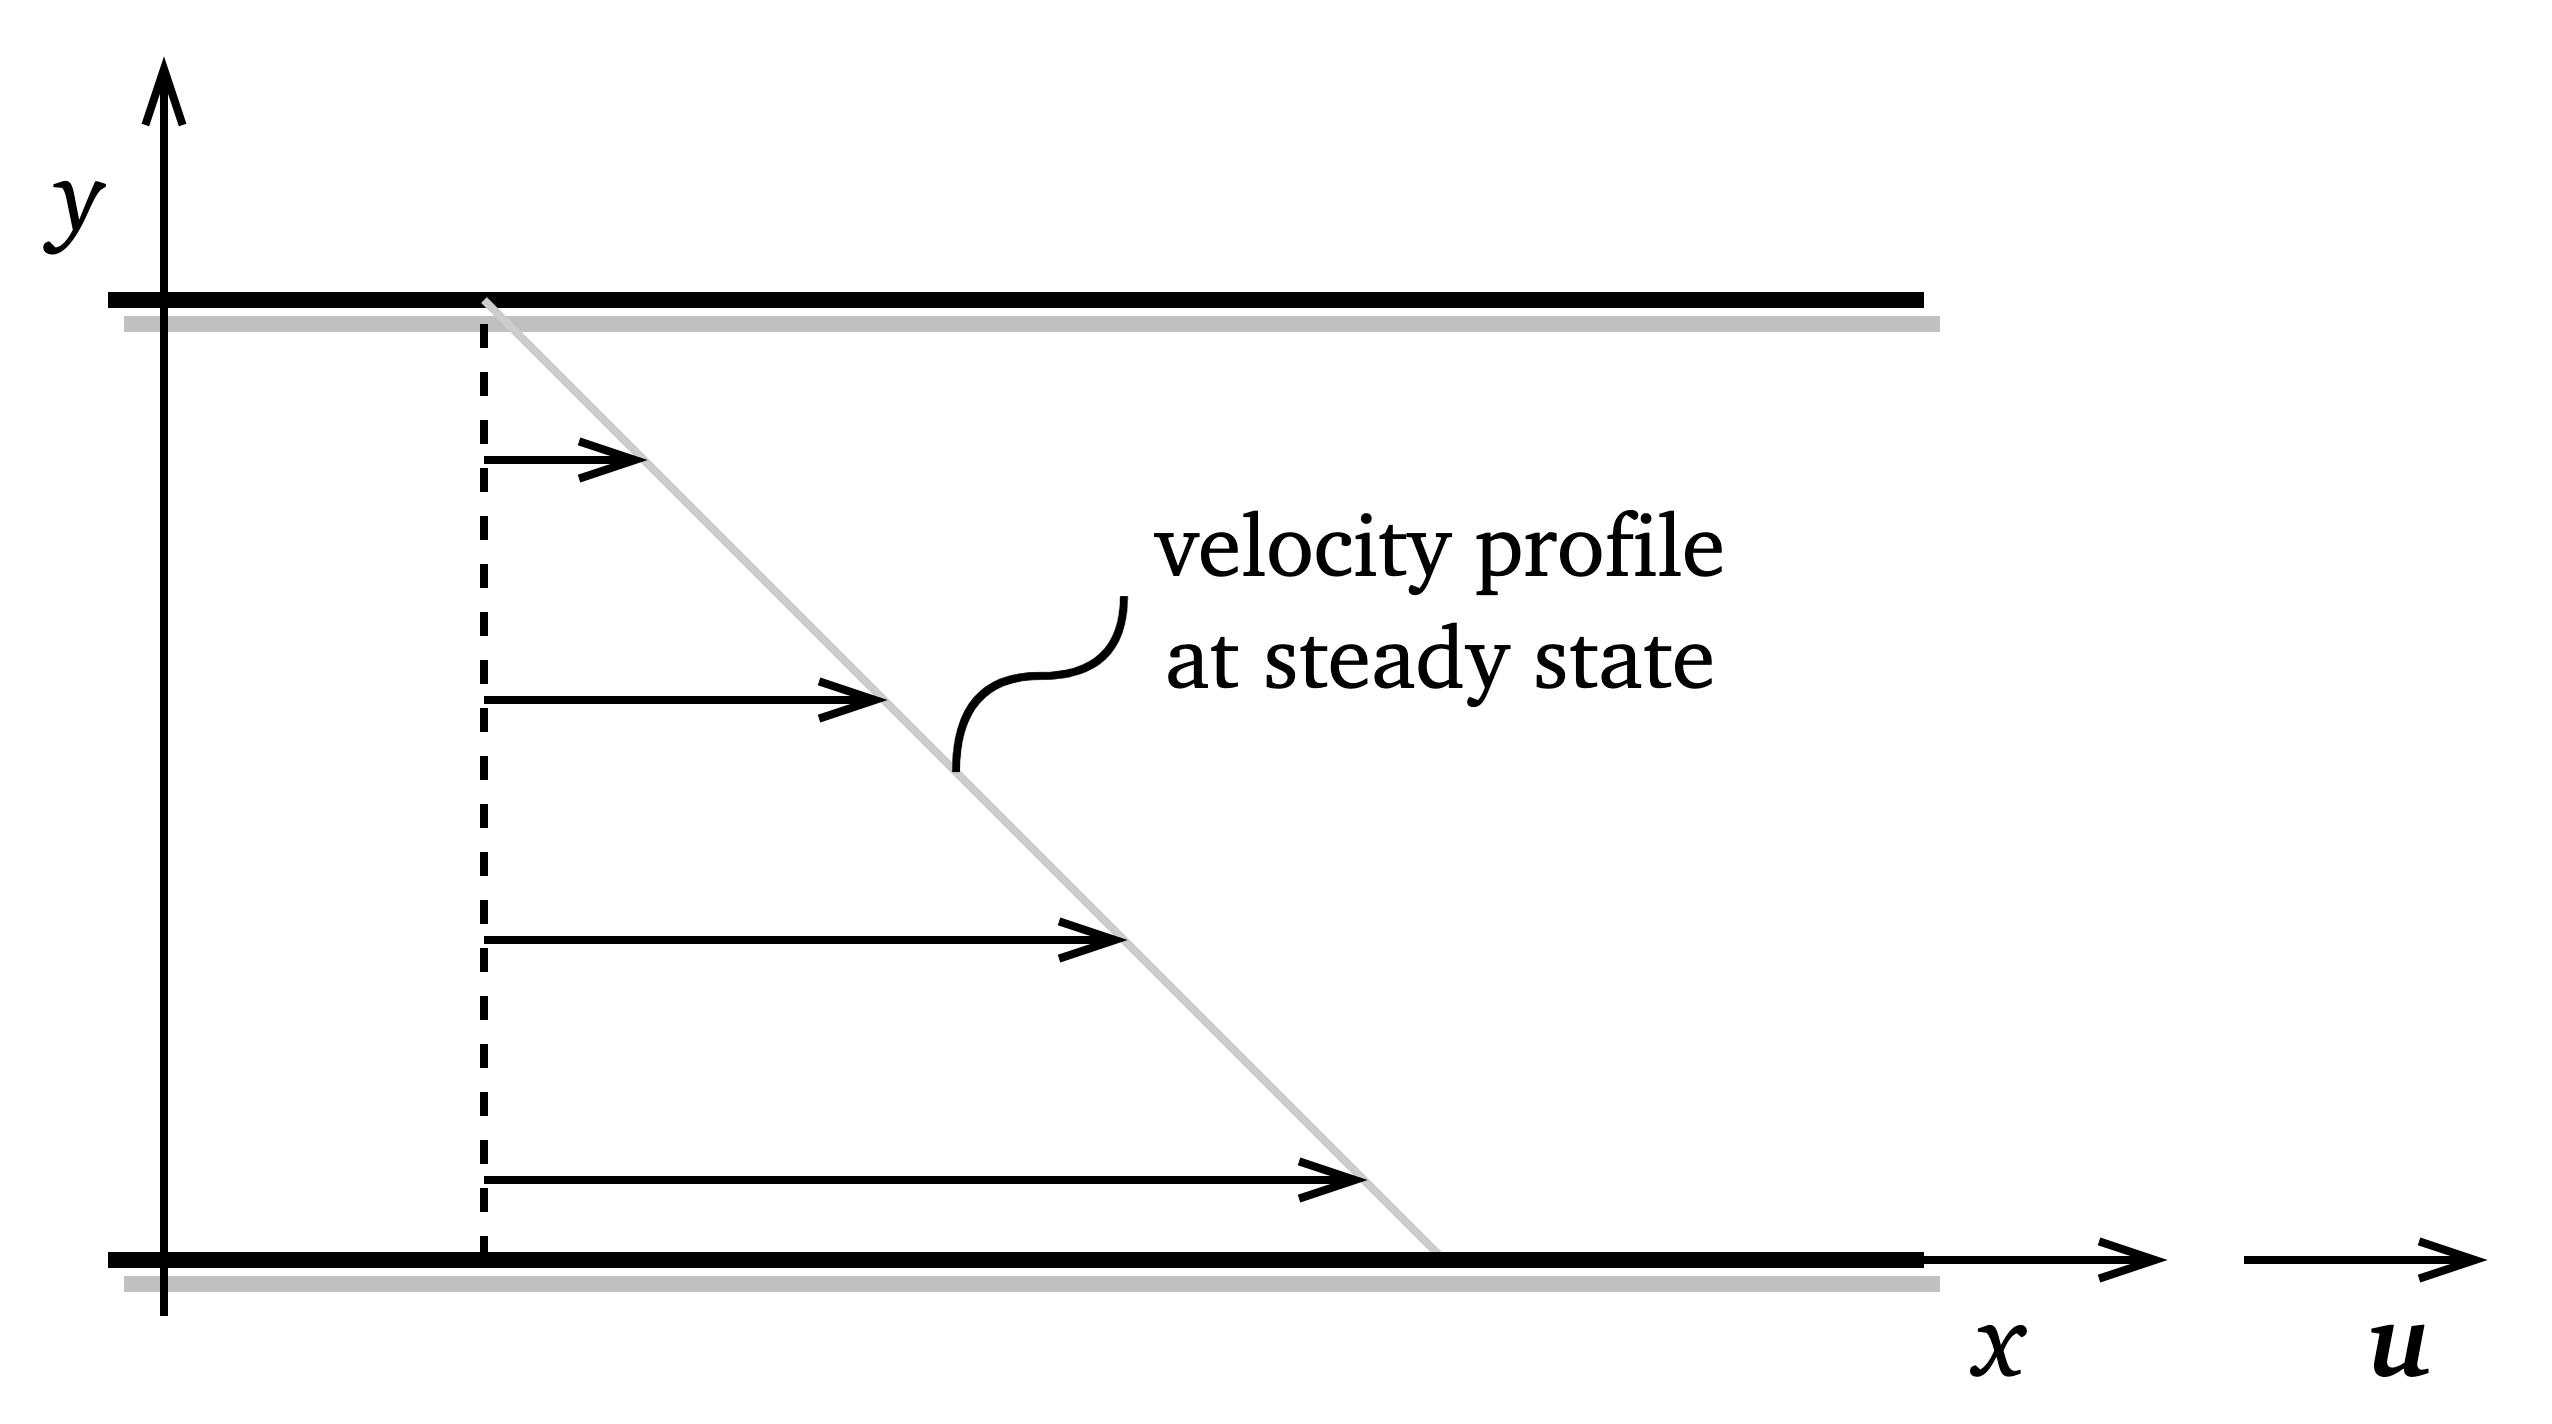
\includegraphics[width=7cm]{couette-flow.png}
\caption{Velocity profile in the Couette flow.}
\label{fig:couette-flow}
\end{figure}
Suppose however, that we start with the initial situation when both plates were stationary and at some moment in time we begin moving the bottom plate reaching the velocity $u$. You may already expect that the moment we started moving the plate something interesting starts to happen in the fluid in-between - it begins moving as well. As the flow develops, the moving plate successively "drags" fluid particles in a layer adjacent to the plate. Once those fluid particles start moving in the positive $x$-direction, that layer of fluid "drags" another layer laying directly on top of it. This "dragging" progresses upward, in the positive $y$-direction, until at the top stationary plate the fluid is stagnant again. After a sufficient amount of time the situation becomes steady - the velocity profile is fully developed and does not change in time. The velocity profile is plotted in Figure \ref{fig:couette-flow} as well. It is a linear function of $y$ but that is something that we will not prove here.

\begin{wrapfigure}{R}{0.1\textwidth}
\centering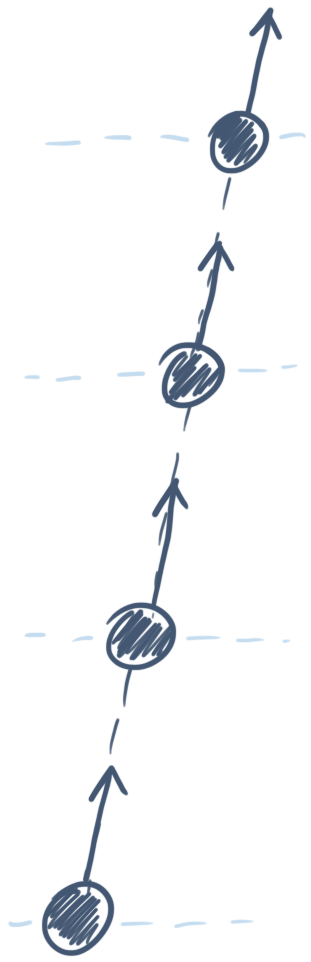
\includegraphics[width=1.8cm]{molecular-collisions.png}
\label{fig:molecular-collisions}
\end{wrapfigure}
If we assume that the fluid flow between plates is laminar we may, perhaps a bit naively, assume that fluid flows in thin "laminates" stacked one on top of the other. Knowing the velocity profile, we know exactly what the velocity of each laminate is (at any position $y$). In general, laminate at a lower $y$ coordinate will have a larger velocity than laminate at a larger $y$ coordinate\footnote{That holds in our case where we assumed that it's the bottom plate that is moving and velocity decreases to zero as $y$ increases. Similar reasoning can be done assuming that the top plate is moving at velocity $u$ and the bottom one is stationary.}.
In Figure \ref{fig:momentum-transport-in-laminates} we have drawn three such laminates.
Knowing the velocities, we also know the momentum carried by each laminate. We will in fact consider specific momentum for the purpose of this discussion which is momentum per unit volume. Let's look at the situation from the perspective of one of the laminates whose $y$-coordinate is simply denoted $y$. Its specific momentum is $\rho \mathbf{u}|_{y}$.  It gains momentum from the faster moving laminate directly below whose specific momentum is $\rho \mathbf{u}|_{y-dy}$. It also looses momentum to the slower laminate directly above it whose specific momentum is $\rho \mathbf{u}|_{y+dy}$. Such "transport" of momentum is in practice possible due to molecular collisions - every collision is an opportunity to exchange momentum. When molecules from one laminate collide with molecules from another laminate, momentum can be transported in the positive $y$-direction. 

\begin{figure}[H]
\centering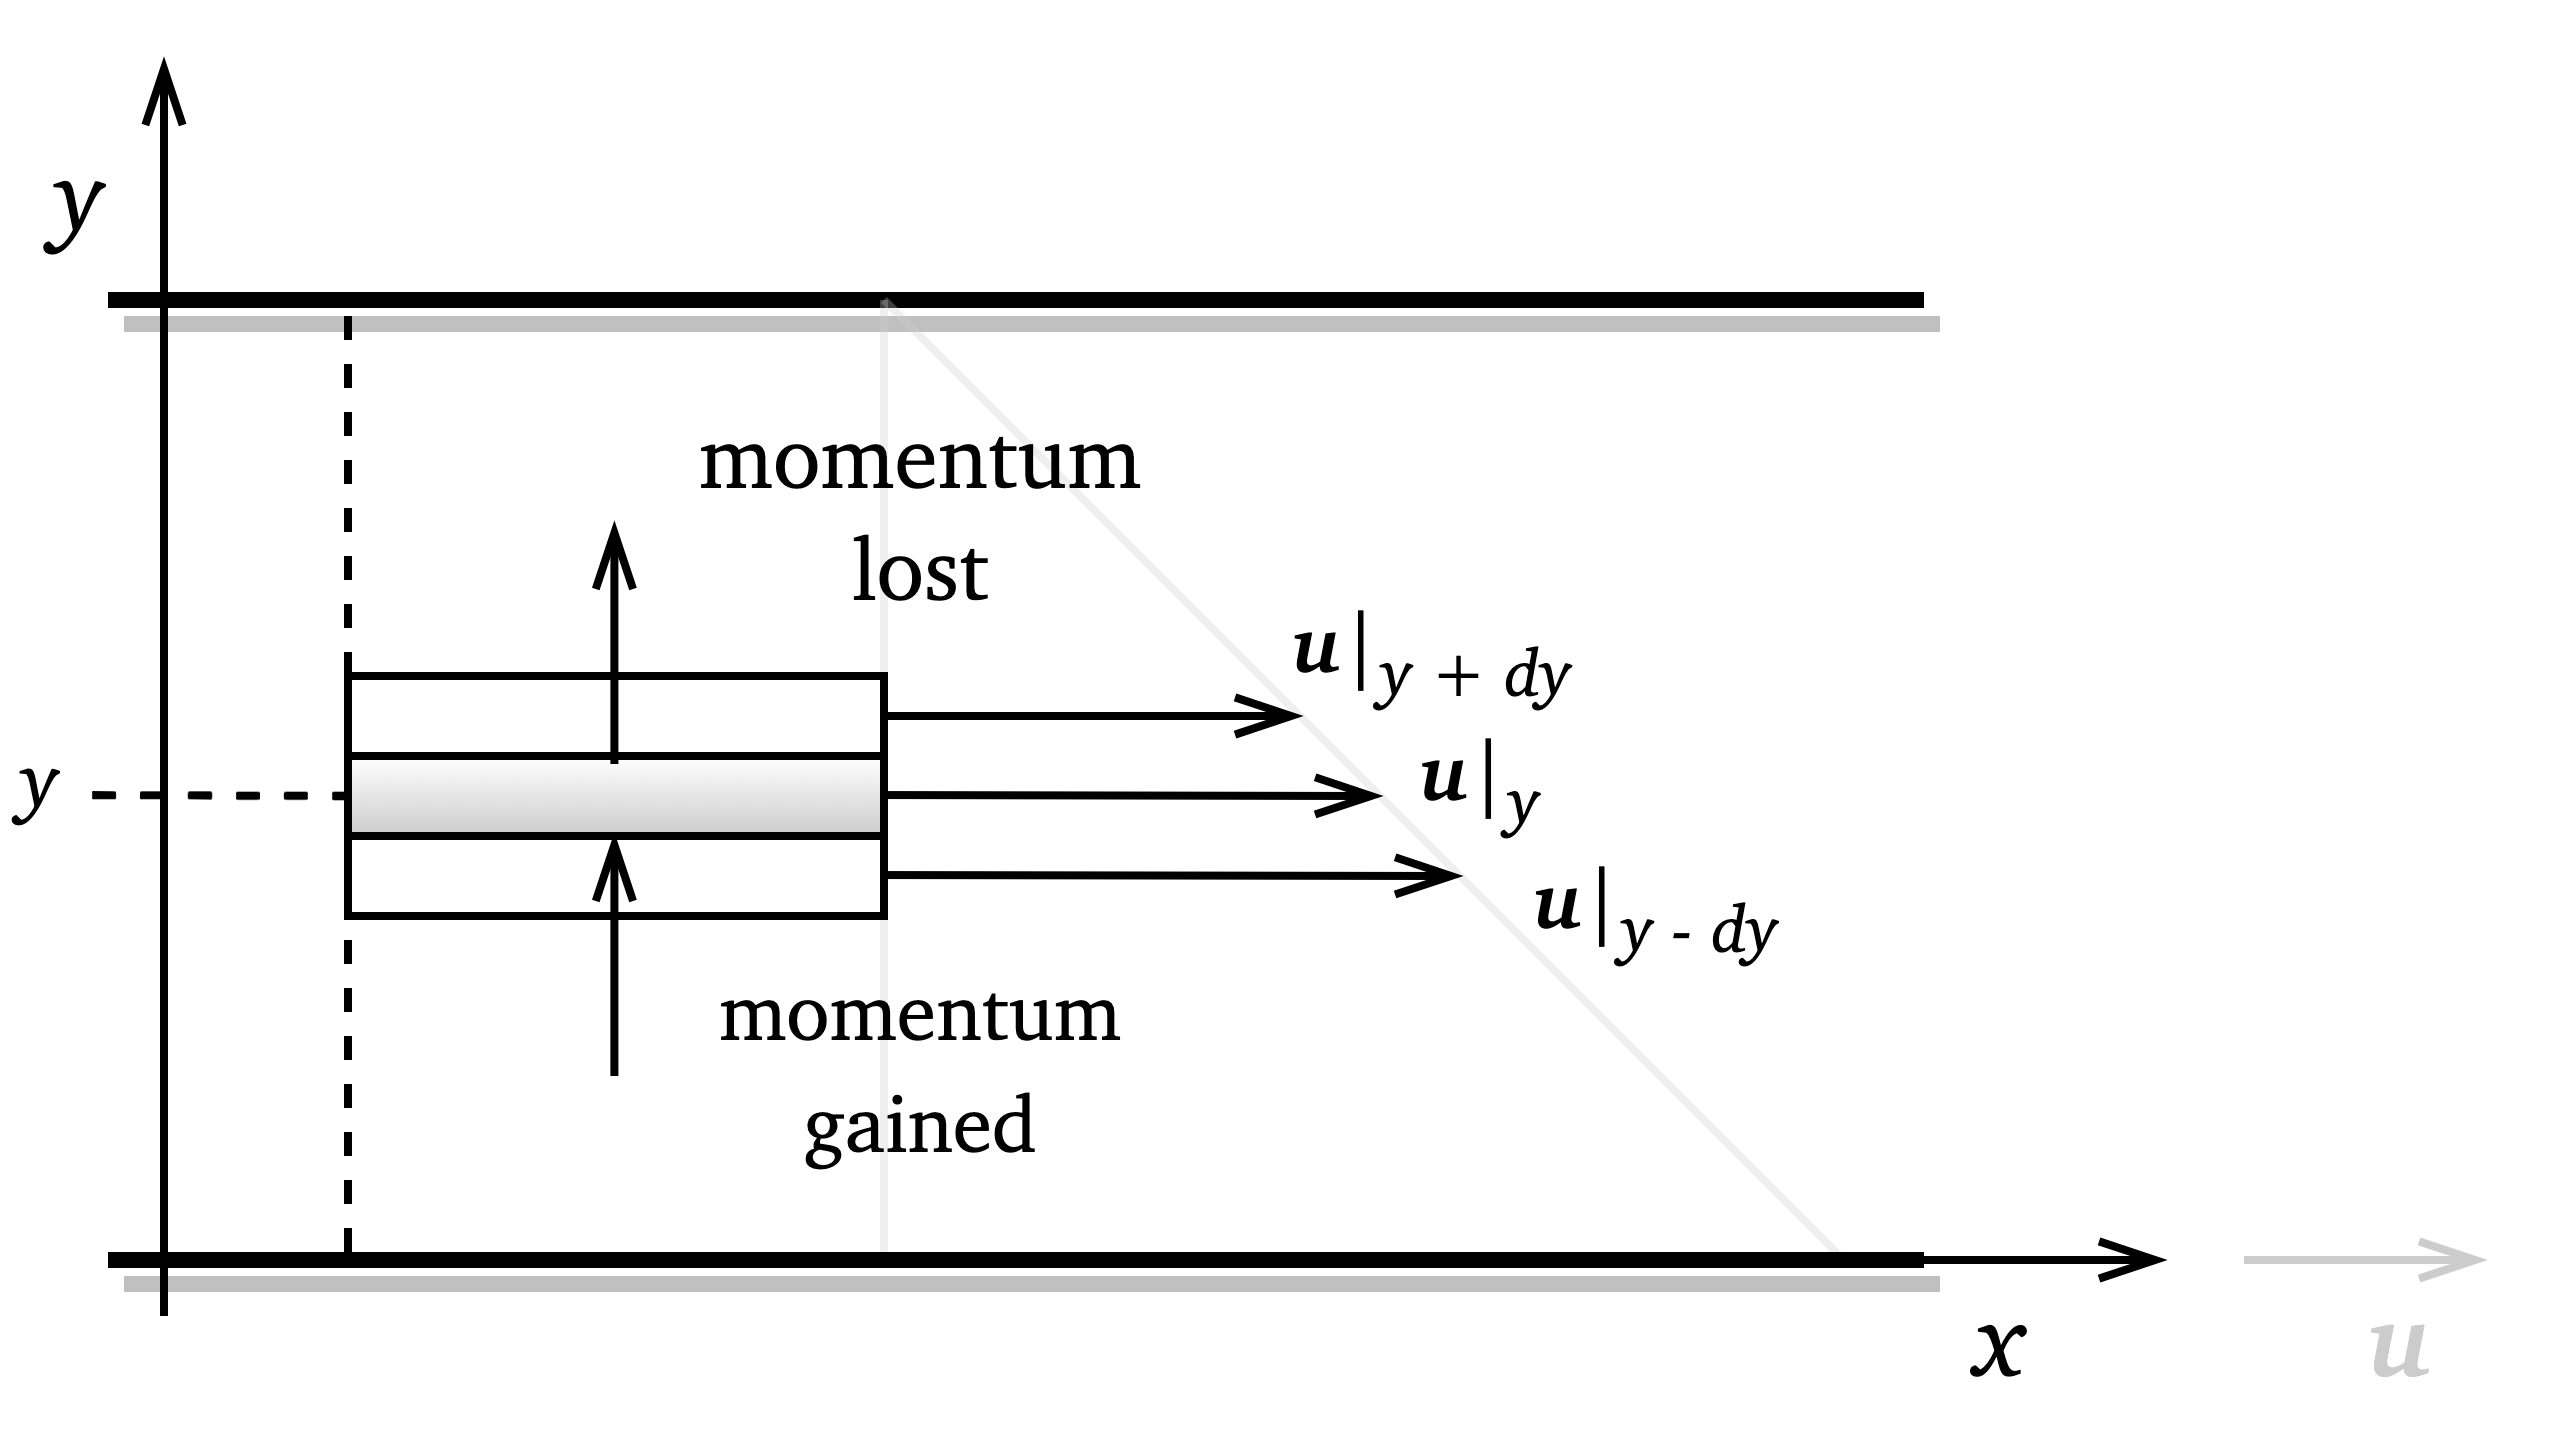
\includegraphics[width=7cm]{momentum-transport-in-laminates.png}
\caption{Transporting momentum between fluid "laminates".}
\label{fig:momentum-transport-in-laminates}
\end{figure}
The "dragging" that we talked about before is thus achieved by momentum transport - a faster moving laminate gives some of its momentum to the slower moving one. Note that this can only happen in the world with friction! Since in fluids friction is characterized by viscosity it becomes clear that viscosity plays a role in transporting momentum\footnote{In a "frictionless world" momentum can still be transported by a fluid, however not by the viscous action.}.

An important concept now emerges. Momentum is a vector quantity that has the direction of the velocity vector. In our simple example of the Couette flow, momentum of every laminate has direction parallel to the $x$-axis (in accordance with the velocity profile). However, as we have reasoned before, the transport of that momentum is happening in the direction parallel to the $y$-axis. This is conceptually presented in Figure \ref{fig:couette-flow-momentum-transport}. 
\begin{figure}[H]
\centering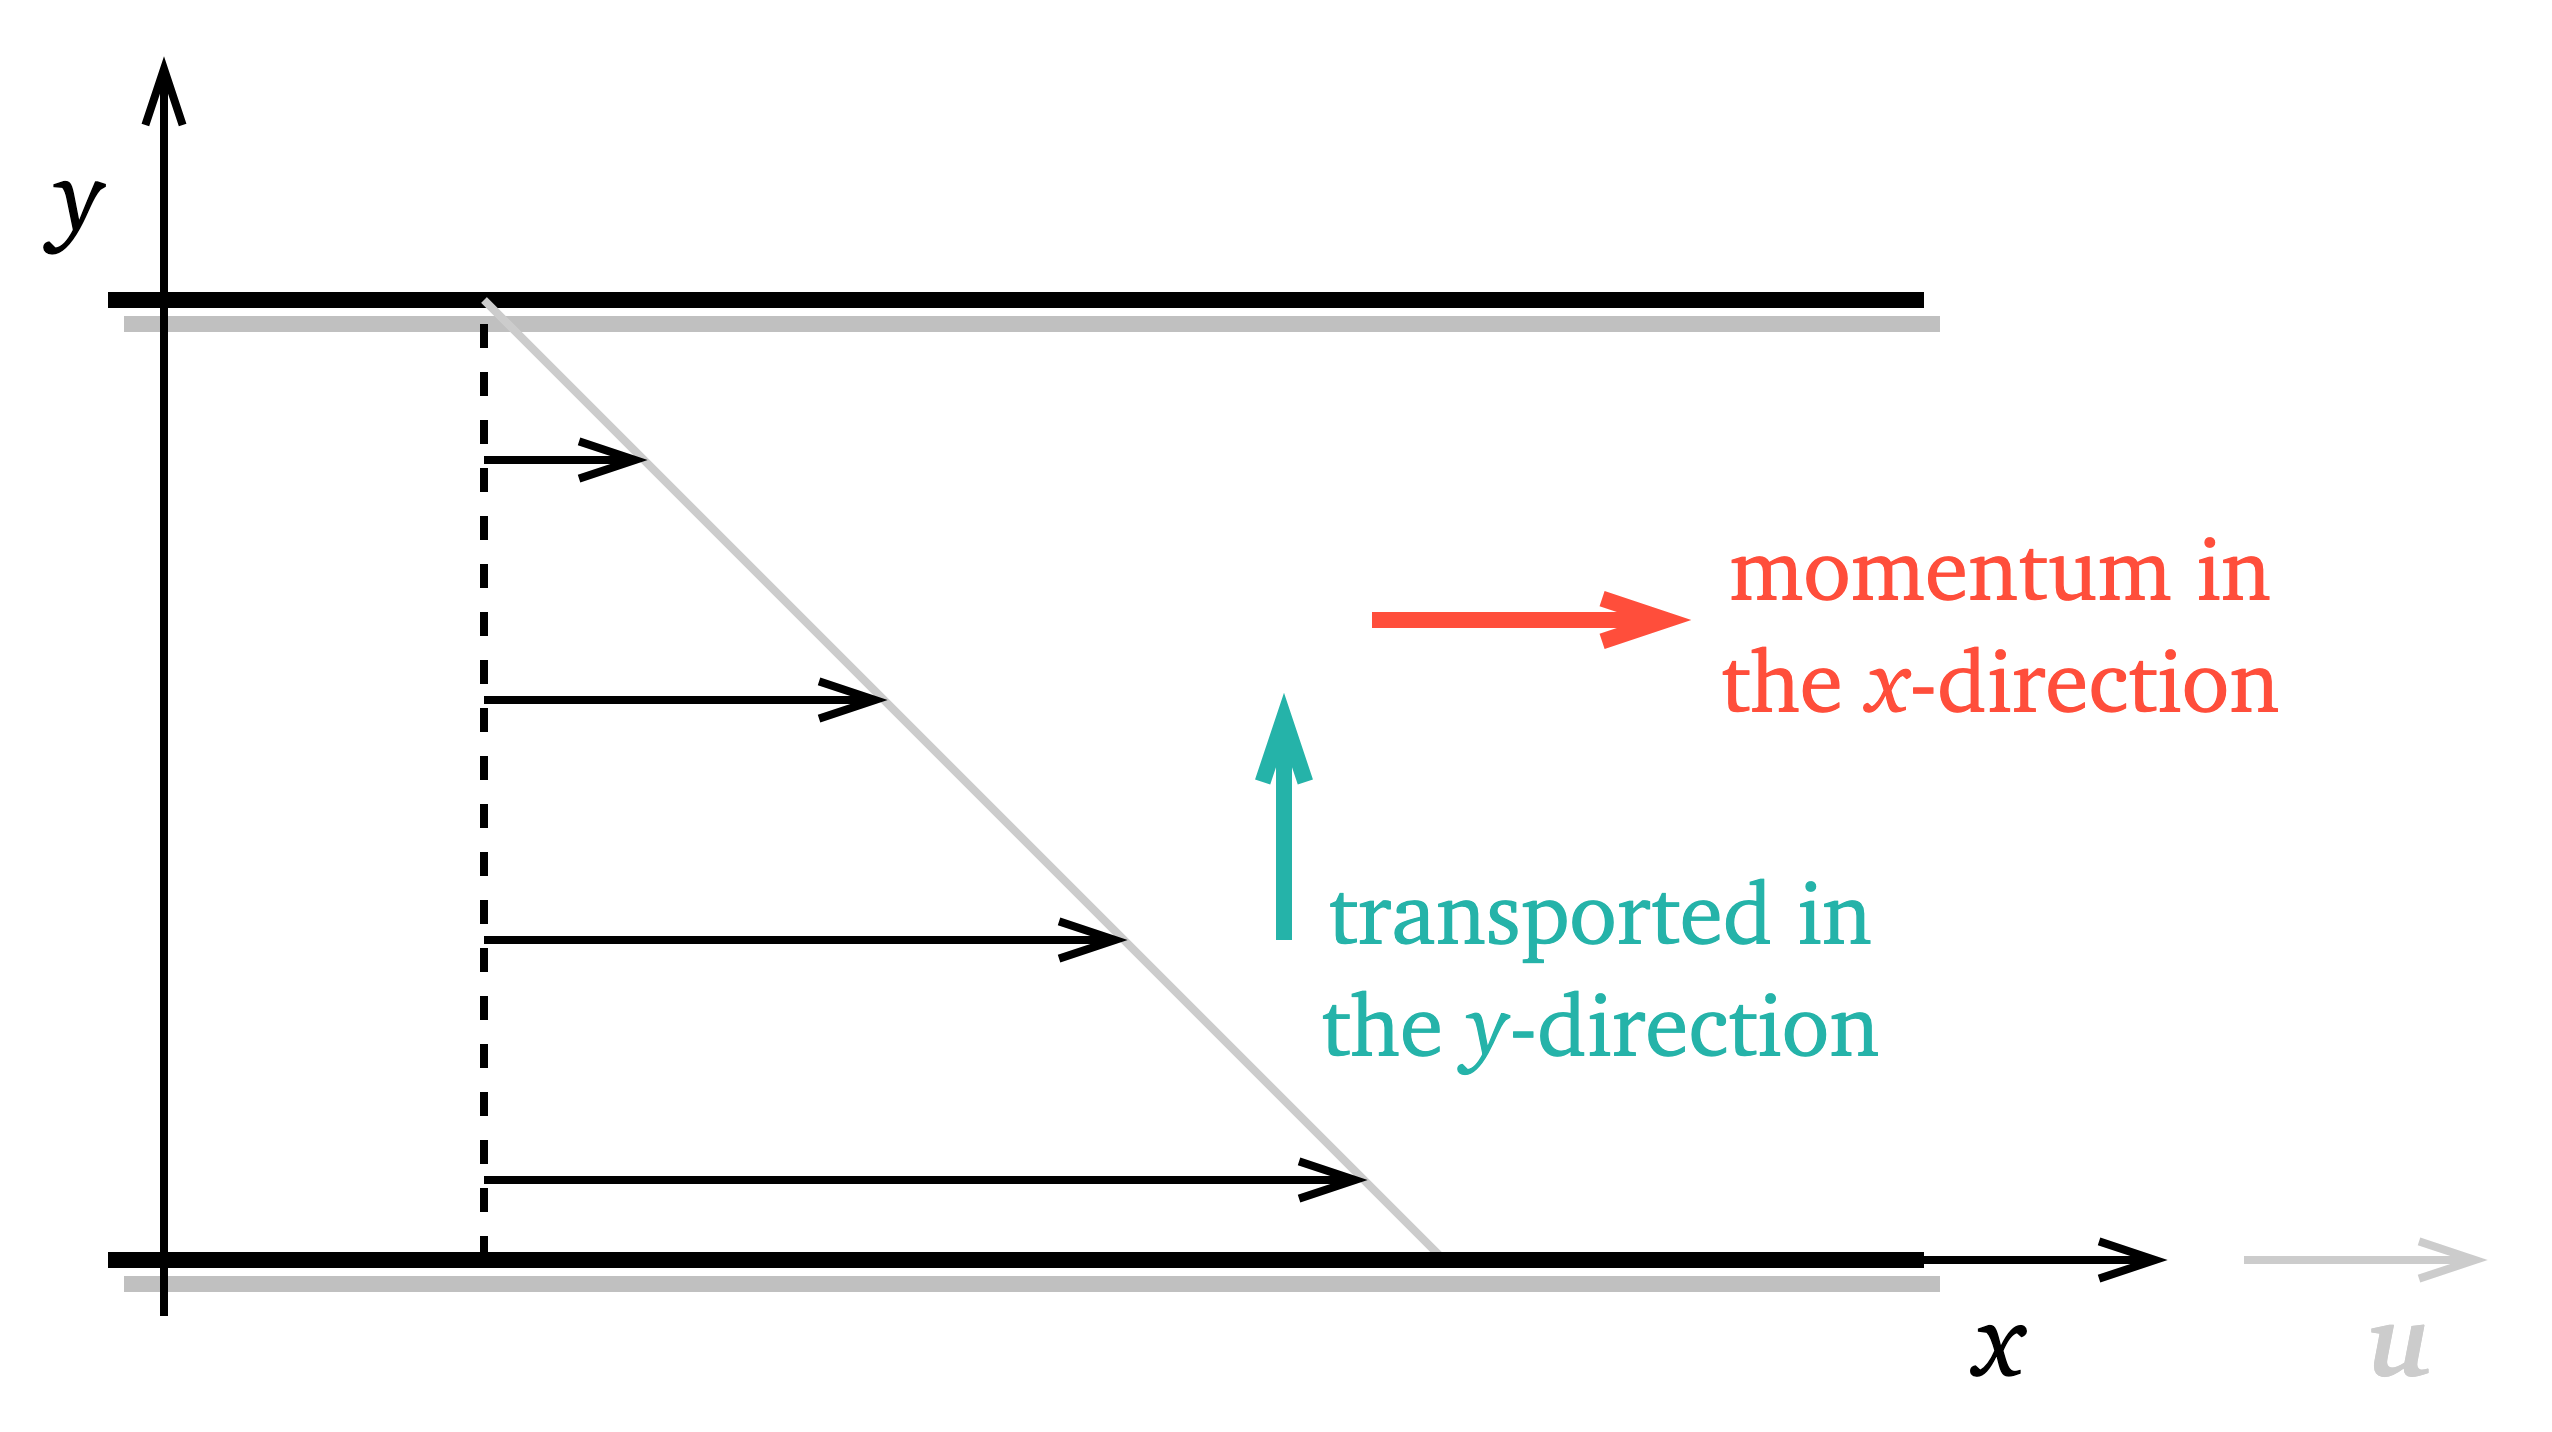
\includegraphics[width=7cm]{couette-flow-momentum-transport.png}
\caption{Momentum transport in a Couette flow.}
\label{fig:couette-flow-momentum-transport}
\end{figure}
\begin{wrapfigure}{L}{0.2\textwidth}
\centering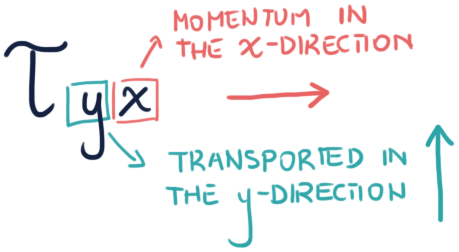
\includegraphics[width=3cm]{tau_y_x.png}
\label{fig:tau_y_x}
\end{wrapfigure}
Such momentum (also called \textit{momentum flux}) is denoted with a symbol $\tau_{yx}$. Notice now that this symbol is carrying information about two directions - one telling us which direction is the momentum vector in and the other telling us which direction that momentum vector is being transported. Tensors are object that keep track of exactly that situation - they allow to associate more than one direction to a physical quantity. In the case of Couette flow considered here, the tensor quantity would be called \textit{rank-2} because that tensor carries information about two directions.

In the most general case - in a 3-dimensional world - momentum vector can be in any of the three directions $x$, $y$ or $z$, transported in any of the three directions $x$, $y$ or $z$\footnote{Can you think of situations when momentum in the $x$-direction is transported in the $x$-direction?}. Tensors allow us to keep track of all those directions as well. For convenience, we often write out the elements of a tensor in a form of a table that resembles a matrix. Unlike in a scalar matrix, this table has additional information "attached" to every element - the directions represented. In Figure \ref{fig:tensor-in-matrix-form} we present an example of the most general tensor of rank two that could represent viscous momentum flux in a 3-dimensional fluid flow.

\newpage

\begin{figure}[H]
\centering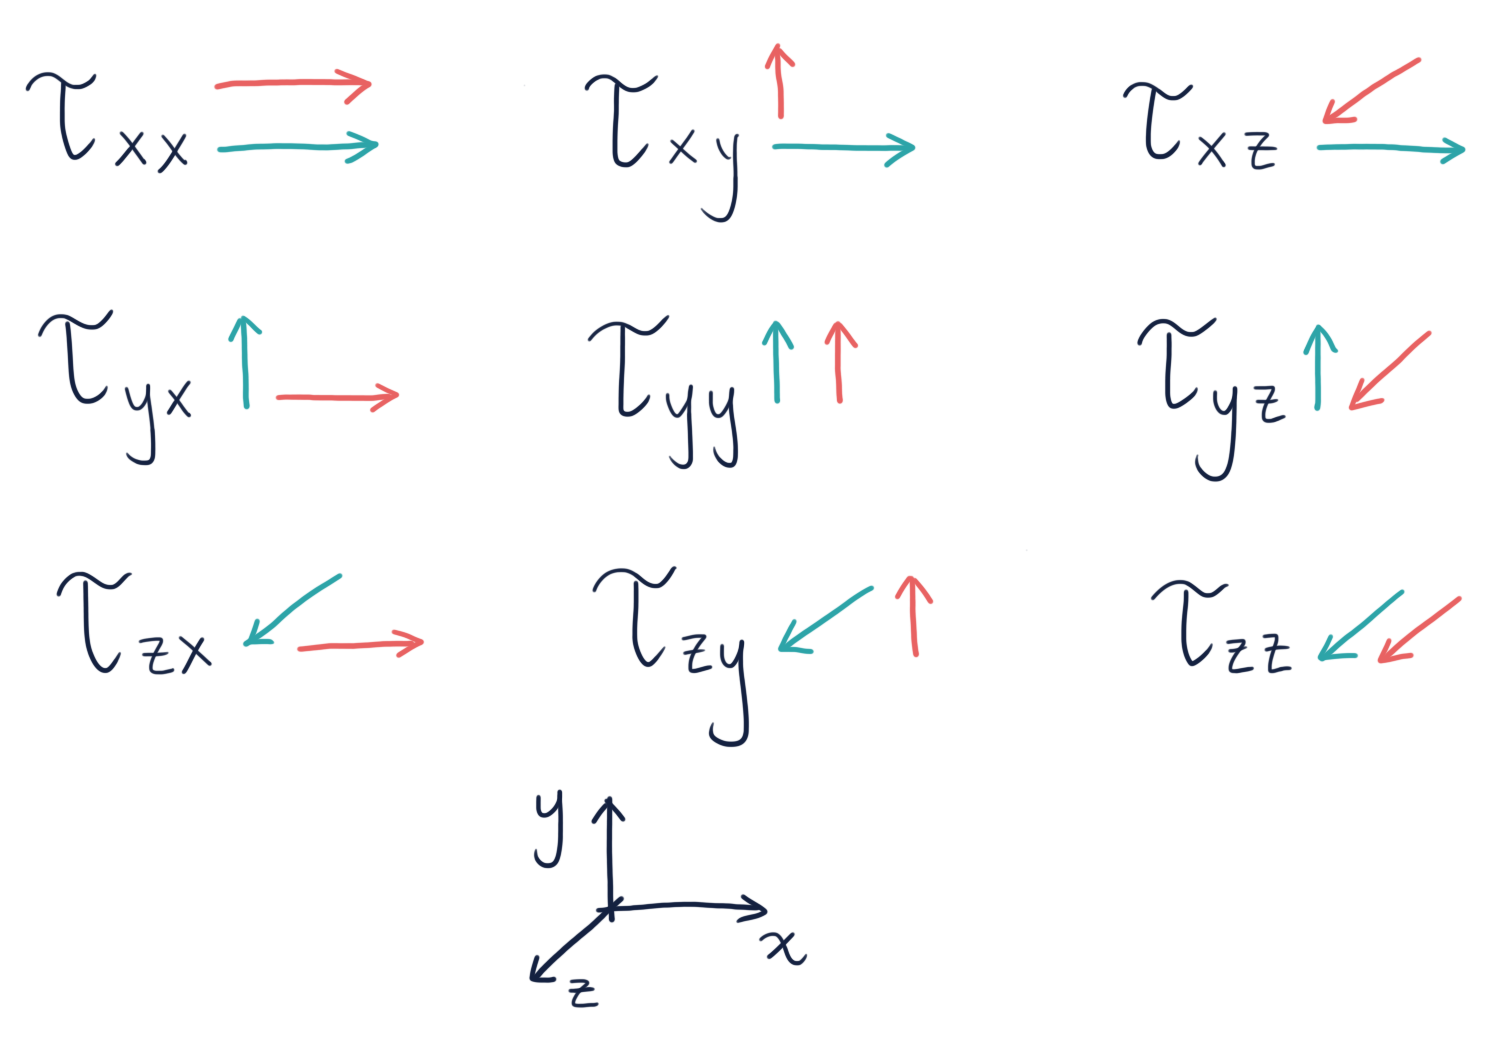
\includegraphics[width=8cm]{tensor-in-matrix-form.png}
\caption{Second order tensor from a 3-dimensional world.}
\label{fig:tensor-in-matrix-form}
\end{figure}











Some say that a good scientific writing that keeps the reader engaged is characterized by a single idea carried over from sentence to sentence that guides the reader through the journey. Hopefully I managed to make this document interesting to you by having an idea transport in the direction downward the paragraphs!


















\thebibliography{}

\bibitem{BSL} R.B. Bird, W.E.Stewart, E.N. Lightfoot, \textit{Transport Phenomena}, John Wiley \& Sons, Inc., 2001

\end{document}